\section{Результаты}
Молекула трифторметанола было оптимизирована методом B3LYP/6-31G. Было предположено, что переходнымм состоянием в барьере поворота вокруг C-O-связи является геометрия, в которой атомы F и H заслонены. После этого была проведена оптимизация в этой точке.

Энергии полученных геометрий приведены ниже: 
\begin{table}[H]
    \caption{Значения составляющих полной энергии ES и TS (в Хартри)} \label{tab:my-table}
        \begin{center}
            \begin{tabular}{|c|c|c|}
            \hline
             & ES & TS \\ \hline
            \begin{tabular}[c]{@{}c@{}}Кинетическая энергия\\ электронов\end{tabular} & 411.356 & 411.351 \\ \hline
            \begin{tabular}[c]{@{}c@{}}Электрон-электронное\\ взаимодействие\end{tabular} & 356.644 & 356.576 \\ \hline
            \begin{tabular}[c]{@{}c@{}}Электрон-ядерное\\ взаимодействие\end{tabular} & -1380.896 & -1380.760 \\ \hline
            \begin{tabular}[c]{@{}c@{}}Ядер-ядерное\\ взаимодействие\end{tabular} & 199.710 & 199.647 \\ \hline
            \textbf{Полная энергия} & \textbf{-413.187} & \textbf{-413.185} \\ \hline
            \end{tabular}
        \end{center}
    \end{table}

Высота потенциально барьера составляет 0.002 Хартри (0.054 eV).

Расчеты проводились при температуре $T = 298.15\ K$. Высота потенциального барьера в 2 раза превышает величину $kT = 0.026\ eV$\footnote{Можно считать, что барьер непреодолим при комнатной температуре, если  его высота более чем на порядок (иногда считают что не на порядок, а в 5 раз) превышает величину $kT$. Если он превышает $kT$, но менее чем на порядок, то говорят, что “барьер преодолим, хотя процесс малоэффективен”.}. Следовательно, барьер преодолим, хотя процесс малоэффективен.

\begin{figure}[H]
\centering
\captionsetup{justification=centering}
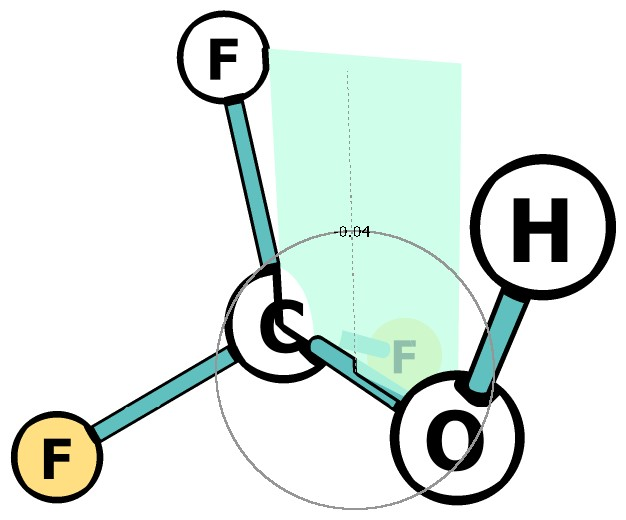
\includegraphics[scale=0.3]{fig/1.jpg}
\caption{Переходным состоянием молекулы трифторметанола является конформация, в которой атомы H и F заслонены.}
\end{figure}
